\section{VHDL Code Analysis}

The VHDL analysis will be done through a \textbf{bottom-up approach}. In the first step the basic components will be analyzed, and through them the Linear Interpolator will be obtained.

\subsection{Ripple Carry Adder}

The Ripple Carry Adder is based on the \textbf{Full Adder}, whose implements the sum between two bits, taking into account a possible carry. The Full Adder is defined as follows:

\begin{figure}[H]
    \centering
    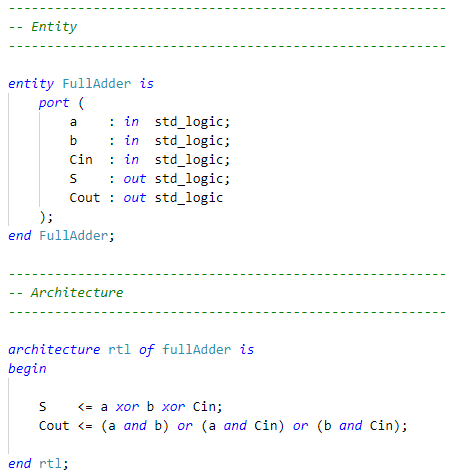
\includegraphics[width=0.5\textwidth]{img/Chapter3/FA.png}
    \caption{Full adder}
    \label{fig:FA}
\end{figure}

So the \textbf{Ripple Carry Adder} consists of a cascade of Full Adder:

\begin{figure}[H]
    \centering
    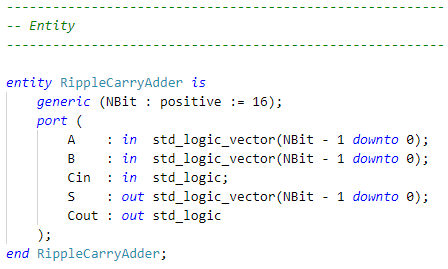
\includegraphics[width=0.5\textwidth]{img/Chapter3/RCA-entity.png}
    \caption{Ripple Carry Adder Entity}
    \label{fig:RCAE}
\end{figure}

\begin{figure}[H]
    \centering
    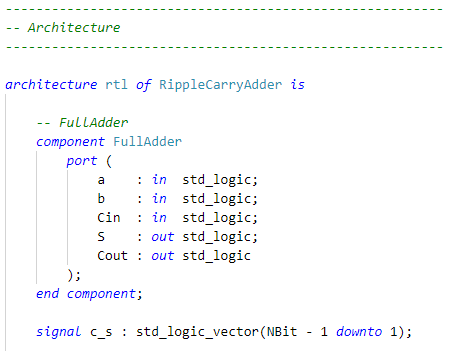
\includegraphics[width=0.5\textwidth]{img/Chapter3/RCA-Architecture1.png}
    \caption{Ripple Carry Adder Component and Signals}
    \label{fig:RCAA1}
\end{figure}

\begin{figure}[H]
    \centering
    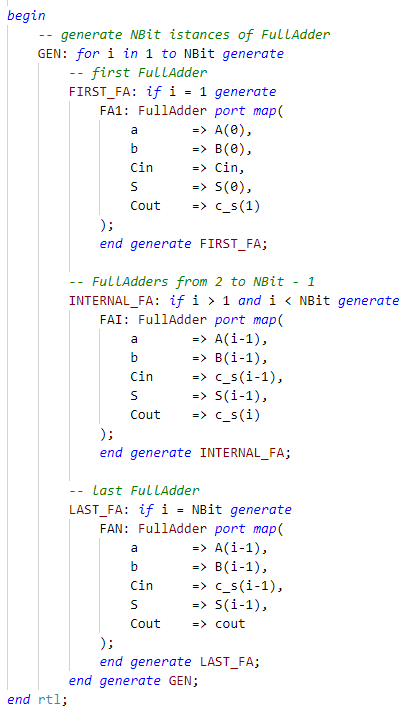
\includegraphics[width=0.5\textwidth]{img/Chapter3/RCA-Architecture2.png}
    \caption{Ripple Carry Adder Internal Architecture}
    \label{fig:RCAA2}
\end{figure}

\subsection{D Flip Flop}

A \textbf{D Flip Flop} involves the use of a low active asynchronous reset. When the clock arrives it stores the new input data only if the enabler is set to one.

\begin{figure}[H]
    \centering
    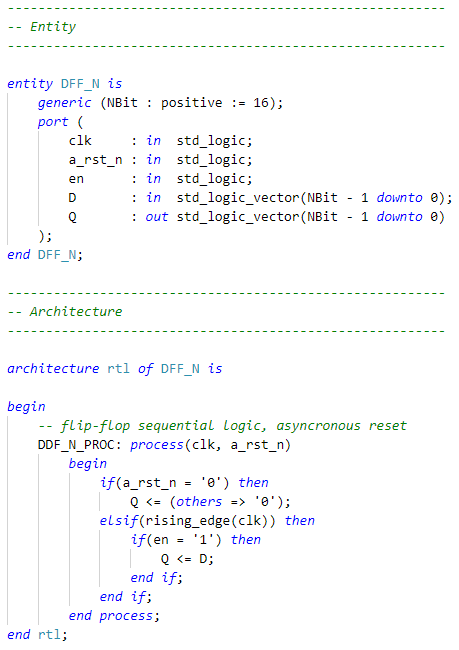
\includegraphics[width=0.5\textwidth]{img/Chapter3/DFF.png}
    \caption{D Flip Flop}
    \label{fig:DFF}
\end{figure}

\subsection{Counter}

The \textbf{Counter} take in input clock and reset, and at every clock cycle it have to increment by one the value that provides in output.

\begin{figure}[H]
    \centering
    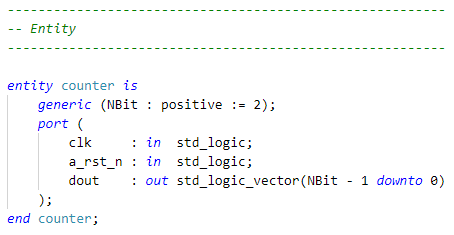
\includegraphics[width=0.5\textwidth]{img/Chapter3/Counter-entity.png}
    \caption{Counter Entity}
    \label{fig:CE}
\end{figure}

Internally it is composed by a register (D Flip Flop) to save and keep stable the output value. The increment operation is implemented through a Ripple Carry Adder. 

\begin{figure}[H]
    \centering
    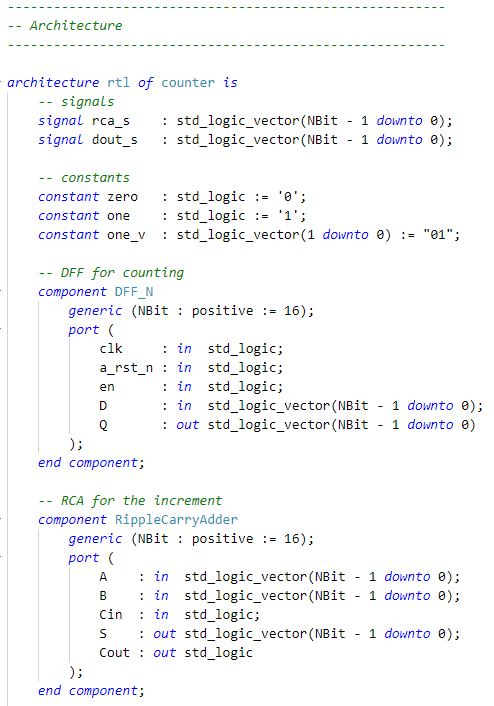
\includegraphics[width=0.5\textwidth]{img/Chapter3/Counter-architecture1.png}
    \caption{Counter Components and Signals}
    \label{fig:CA1}
\end{figure}

The register's output returns in feedback to the Ripple Carry Adder the sums it to one.

\begin{figure}[H]
    \centering
    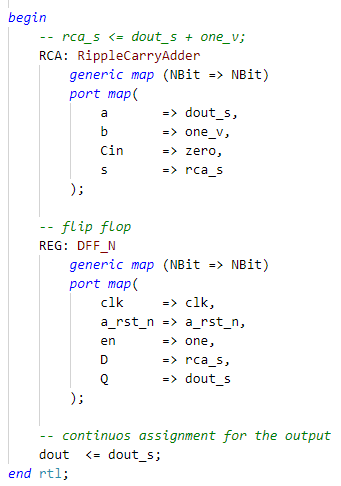
\includegraphics[width=0.4\textwidth]{img/Chapter3/Counter-architecture2.png}
    \caption{Counter Internal Architecture}
    \label{fig:CA2}
\end{figure}

\subsection{Combinational Network}

The \textbf{Combinational Network} follows the structure described in the section 2.2.

\begin{figure}[H]
    \centering
    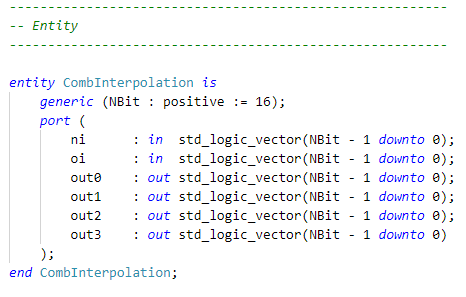
\includegraphics[width=0.5\textwidth]{img/Chapter3/CombInterp-entity.png}
    \caption{Combinational Network Entity}
    \label{fig:CNE}
\end{figure}

As regards the signals, the first four in figure \ref{fig:CNA1} need to implement the divisions by power of two, so they are the signals used by the Ripple Carry Adders to compute the resulting signals.

\begin{figure}[H]
    \centering
    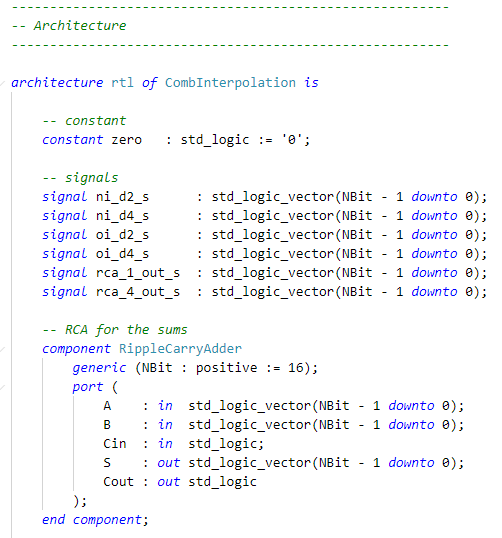
\includegraphics[width=0.5\textwidth]{img/Chapter3/CombInterp-architecture.png}
    \caption{Combinational Network Components and Signals}
    \label{fig:CNA1}
\end{figure}

The next part implements the calculations of the signals described above ($\frac{y_{n+1}}{4}, \frac{y_{n+1}}{2}, \frac{y_n}{4}, \frac{y_n}{2}$). In fact, a single bit shift to right is carried  out to implement the division by two, ad of two bit to implement the division by four.

\begin{figure}[H]
    \centering
    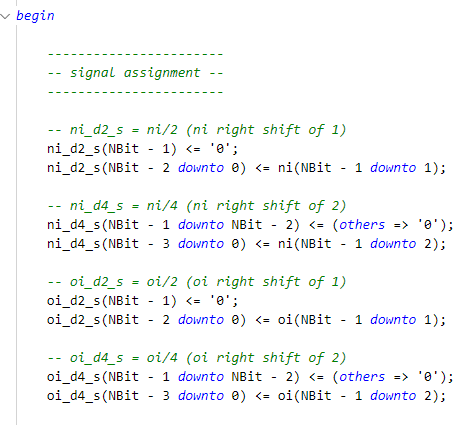
\includegraphics[width=0.5\textwidth]{img/Chapter3/CombInterp-shift.png}
    \caption{Combinational Network Shift bit a bit}
    \label{fig:CNA2}
\end{figure}

The second part of architecture, instead, implements the network described by the figure \ref{fig:OutputSignalsCalc}, that is a composition of five  Ripple Carry Adders, which sums the four signals obtained by the shifts.

\begin{figure}[H]
    \centering
    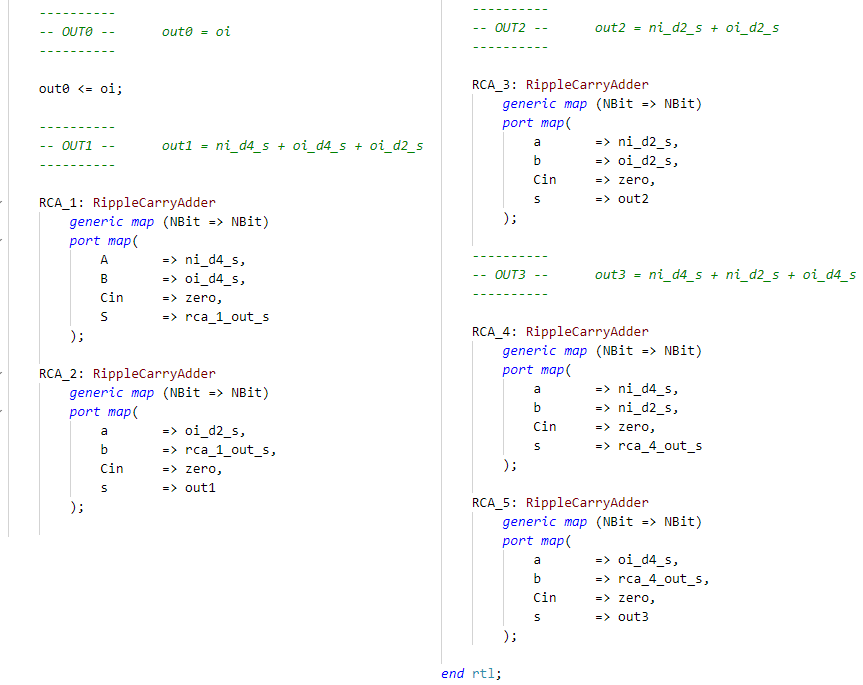
\includegraphics[width=0.8\textwidth]{img/Chapter3/CombInterp-out.png}
    \caption{Combinational Network Output}
    \label{fig:CNA3}
\end{figure}

\newpage

\subsection{Linear Interpolator}

As said before, the \textbf{Linear Interpolator} takes a signals in input and provides in output another signals.

\begin{figure}[H]
    \centering
    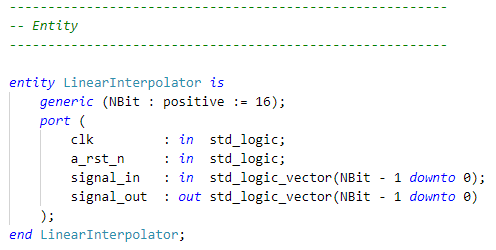
\includegraphics[width=0.5\textwidth]{img/Chapter3/LinearInterpolator-entity.png}
    \caption{Linear Interpolator Entity}
    \label{fig:LIE}
\end{figure}

The Linear Interpolator contains all the previous circuits, so Ripple Carry Adders, D Flip Flops and the Combinational Network.

\begin{figure}[H]
    \centering
    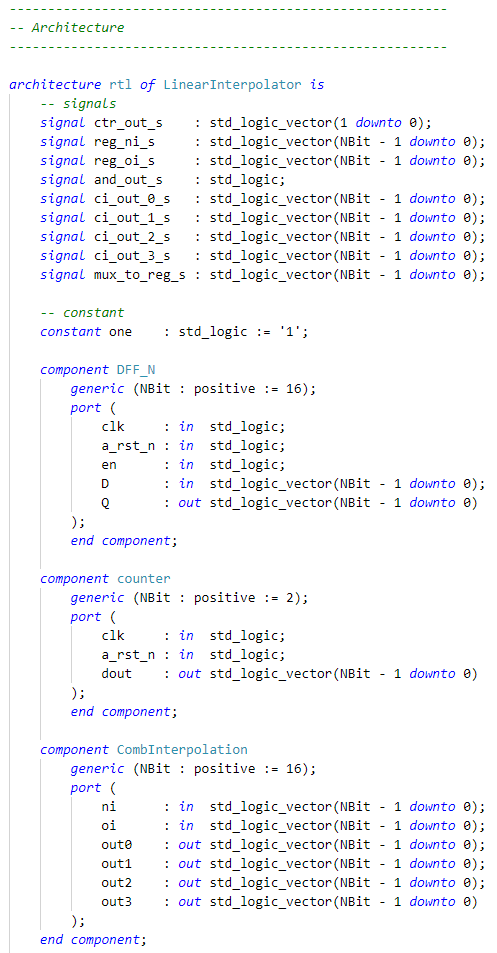
\includegraphics[width=0.45\textwidth]{img/Chapter3/LinearInterpolator-architecture1.png}
    \caption{Linear Interpolator Entity}
    \label{fig:LIA1}
\end{figure}

\textit{REG\_OI} and \textit{REG\_NI} (that are two D Flip Flop), implements the Input Network. In addition to them there is the Counter, whose output go in input to an AND port, implemented by the signal and\_out  \_s. This single bit signal is used as enabler by \textit{REG\_OI} and \textit{REG\_NI}.

The output signals of this two registers are the inputs for the Combinational Network that provides in output the four computed signals. These obtained signals go in input to a Multiplexer, whose output is controlled by the output of the Counter.

The combination between Multiplexer and the register that memorizes its output (\textit{REG\_OUT}) represent the Output Network.

\begin{figure}[H]
    \centering
    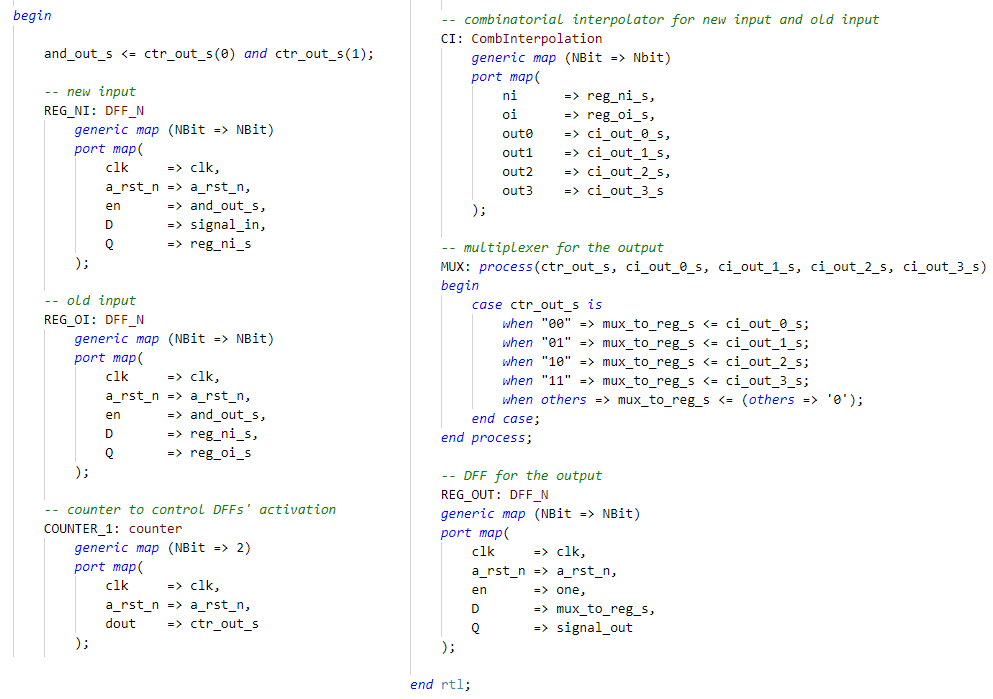
\includegraphics[width=1\textwidth]{img/Chapter3/LinearInterpolator-architecture2.png}
    \caption{Linear Interpolator Entity}
    \label{fig:LIA2}
\end{figure}